\section{Illustrative scenarios}
\label{sec:study}

In this section we present two illustrative scenarios, using census data from
the United States~\citep{nhgis} and
Canada\footnote{\url{http://datacentre.chass.utoronto.ca/census/}}, tabulated by
CTs,  from 1970 to 2010. 

The prototype interface allows access to 41 regions, 29
in the US and 12 in Canada. New York City was split into its boroughs to avoid
memory crashes on the client browser due to the high number of CTs.  We used
five aspects for the USA: Education level, Family income, Marital status,
Occupation, and Race; and seven for Canada: Age, Education level, Home language,
Household Income, Marital status, Occupation, Place of birth, and Religion. The supplementary material contains the details of
which census columns were used for each aspect. 



\unsure{CHECK}\revision{1.12.(1-5)}{These results are meant to demonstrate the
utility of the interface for understanding the evolutionary dynamics of urban
neighbourhoods. They also show the face validity of the results generated by our
novel network-based approach. While our method does not require geographic harmonisation, it does however require matching
the variables over time. This is (currently) a painstaking, manual process, and the current version of the interface remains somewhat limited. For example, we selected a minimal set of
aspects for each country, which are not necessarily similar to each other, or
similar to studies in the current literature. Income moreover is slightly inaccurate,
even though we did correct for official inflation. We grouped the original
ranges into three larger ranges, but they do not match precisely. In addition, the US data labelled "2010" is  not from the decennial census, but from the ACS 2006-2010, somewhat compromising the temporal
stability of the data. Further, the regions selected do not correspond to any
pre-defined regions (metros, cities, census areas), but to somewhat arbitrary
regions defined around a location of interest, making direct comparisons harder.
Taken together, these factors would no doubt require caveats for 
a substantive study using the current prototype version of the interface. Nevertheless, in the present context we find that the interface results are well-aligned
with several other studies, illustrating the robustness of our approach to
imperfect conditions. }

\subsection{Chicago}
Our first scenario examines Chicago, using an arbitrary region larger than the
administrative borders. Its demographic composition is well explored in the
literature, with reports of racial divide and
gentrification~\citep{Delmelle2016,Delmelle2017,Hwang2014}, so we expect our
results to contain stable regions where the Race aspect is relevant, and some
degree of population change, with increasing income and education levels. 


The initial state of the prototype is illustrated in Figure~\ref{fig:ui}. The
first step is to identify \textit{what} the clusters consist in. To do so, we
examine the compositions of each cluster from the boxplots. Orange is associated
with majority of White population, green with majority Black, and purple with
higher proportion of four years of college or more (high education level). The
expanded version of the boxplots for the purple cluster shows a higher income
level and majority of occupations in administrative jobs. The purple cluster
therefore could be described as gentrified regions.


The trajectories plot shows \textit{how} clusters have changed over time.  For
example, it illustrates the process of gentrification, also illustrated in
Figure~\ref{fig:chiWorkflow}, with the purple cluster progressively absorbing
regions from the orange cluster (White). This corroborates results from the
literature reporting that Black neighbourhoods are less likely to
gentrify~\citep{Hwang2014}. The transition matrix provides more details, showing
that around one percent of all regions that became purple at any time
transitioned from the green cluster (Black population), while nine percent were
previouly associated with the orange cluster (White). Next, we select the region
that is gentrified in 2010, by clicking on the corresponding rectangle in the
trajectories plot, updating the information on the maps and the details portion
of the interface.

The maps show \textit{where} these processes are occurring, by highlighting the
corresponding regions. The spatial pattern is clear, corresponding exactly to
previous findings in the literature based upon harmonisation~\citep{Hwang2014}.
Further, we can also identify the regions that gentrified earlier on the small
maps that depict the involved regions over time. Finally, we can examine
\textit{who} is driving these changes. Since the most relevant aspect is
Education, specifically "Four or more years of college", we can expand the
details of this aspect, as illustrated in the rightmost portion of
Figure~\ref{fig:chiWorkflow}, which is increasing for the whole city (grey
band), but faster and to a higher level in this region (black band).

\unsure{CHECK - maybe add what/how/where/who to figure 5?}

\begin{figure*}
    \centering
 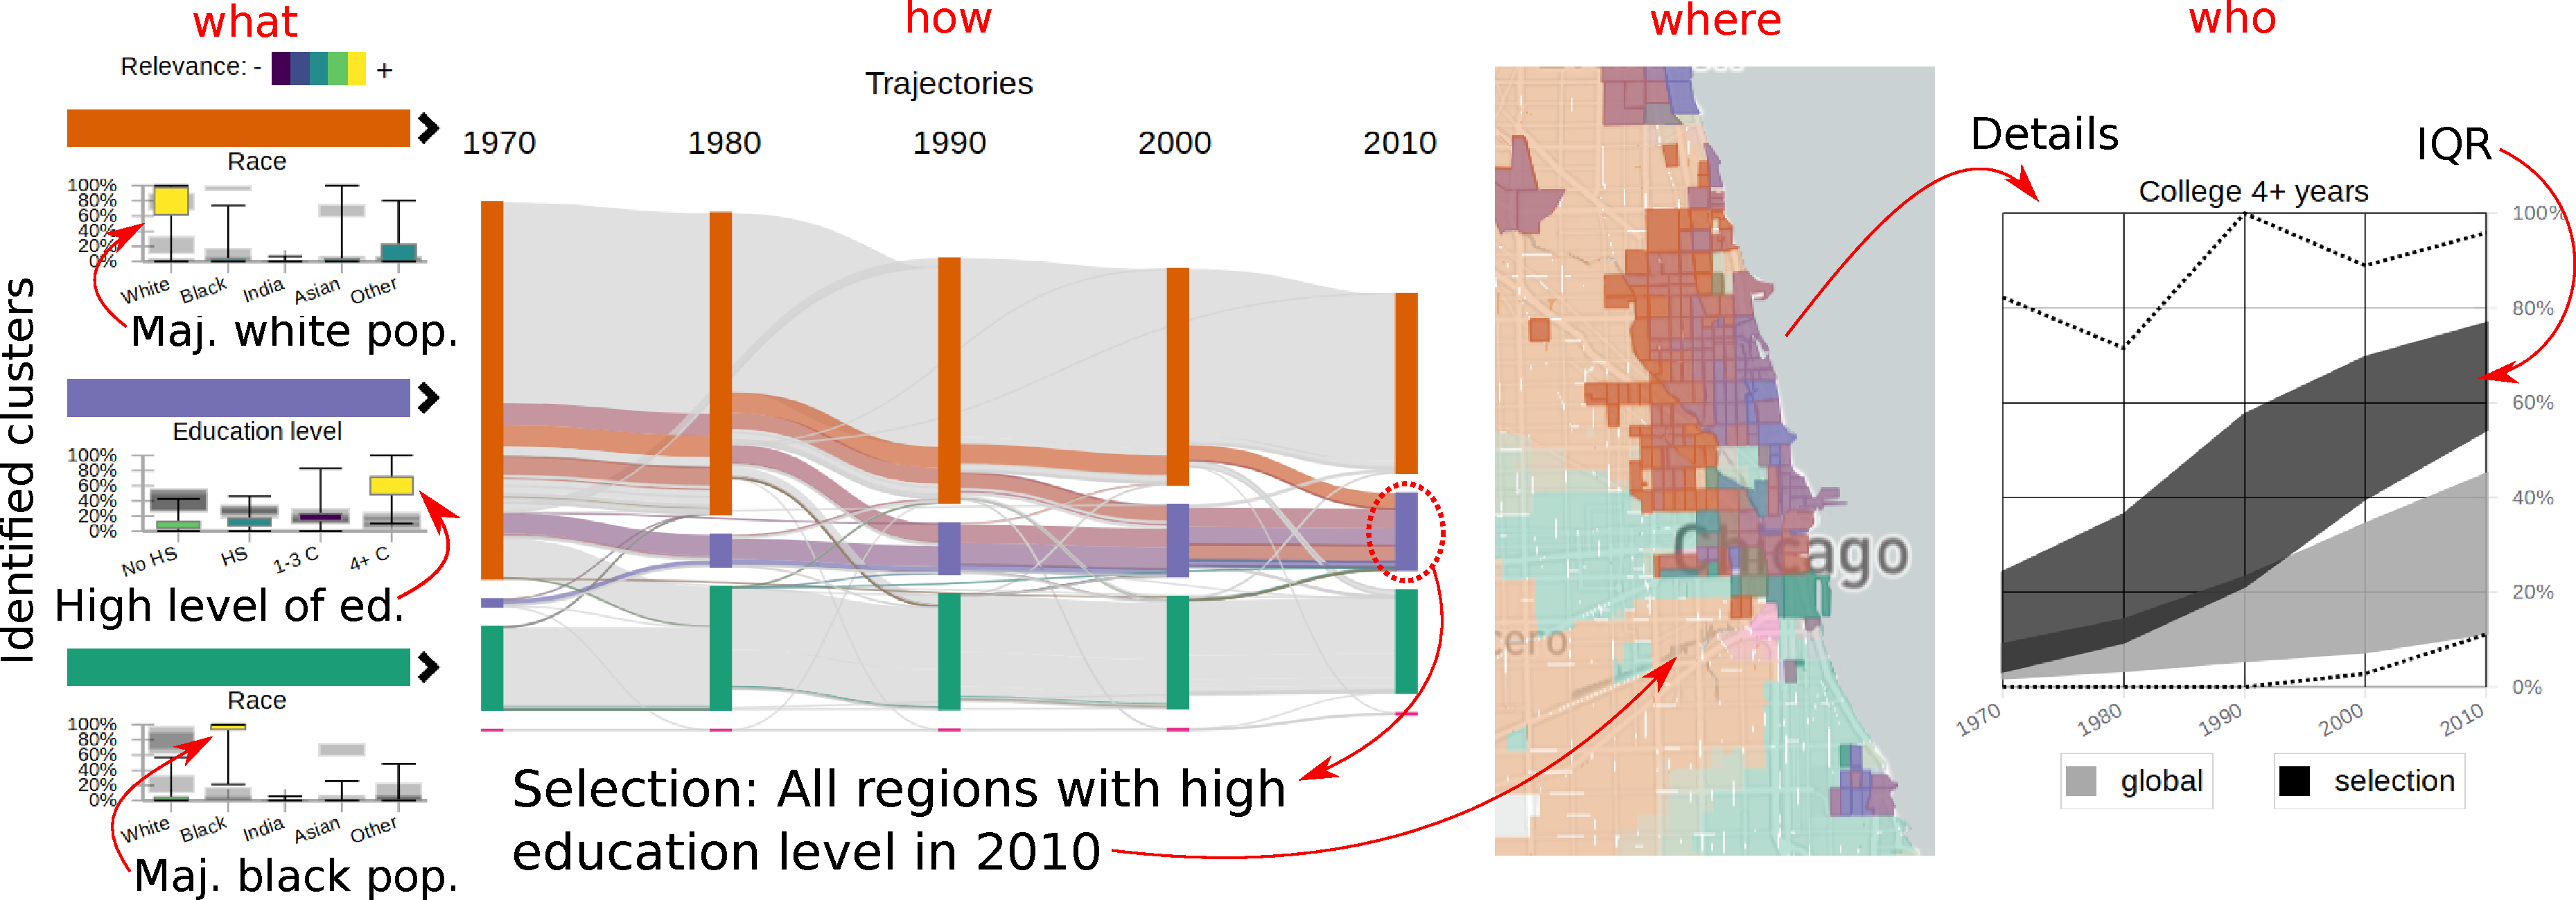
\includegraphics[width=0.9\linewidth]{newTeaser.pdf}
 \caption{Workflow to discover gentrification in Chicago: the purple cluster
 corresponds to high education / income. Its population is increasing over time,
 absorbing from the majority White cluster (orange). By selecting the purple
 cluster in 2010, the region is highlighted in the maps. The proportion of
 people with 4+ years of college is increasing in the whole city (grey IQRs),
 but significantly more in this region (black).\label{fig:chiWorkflow}}
\end{figure*}



\subsection{Toronto}

We consider a region that corresponds approximately to the administrative border
of the current city of Toronto, using all seven available aspects with equal
weights. While Chicago was fairly stable, Toronto is known to be a more dynamic
and diverse city, with significant and increasing immigrant
population~\citep{hulchanski2007three,Fong2011}, especially
Asian~\citep{Fong2003}. Toronto is also known for a stable and well defined
Jewish community~\citep{Harold2018, Fong2011}. Therefore, we expect \revision{1.14}{a}
combination of stable and dynamic regions on the results, with Place of Birth,
Home Language, and Religion identified as relevant aspects. The results are
summarised in Figure~\ref{fig:to}, considering eight clusters.

\begin{figure}
    \centering 
    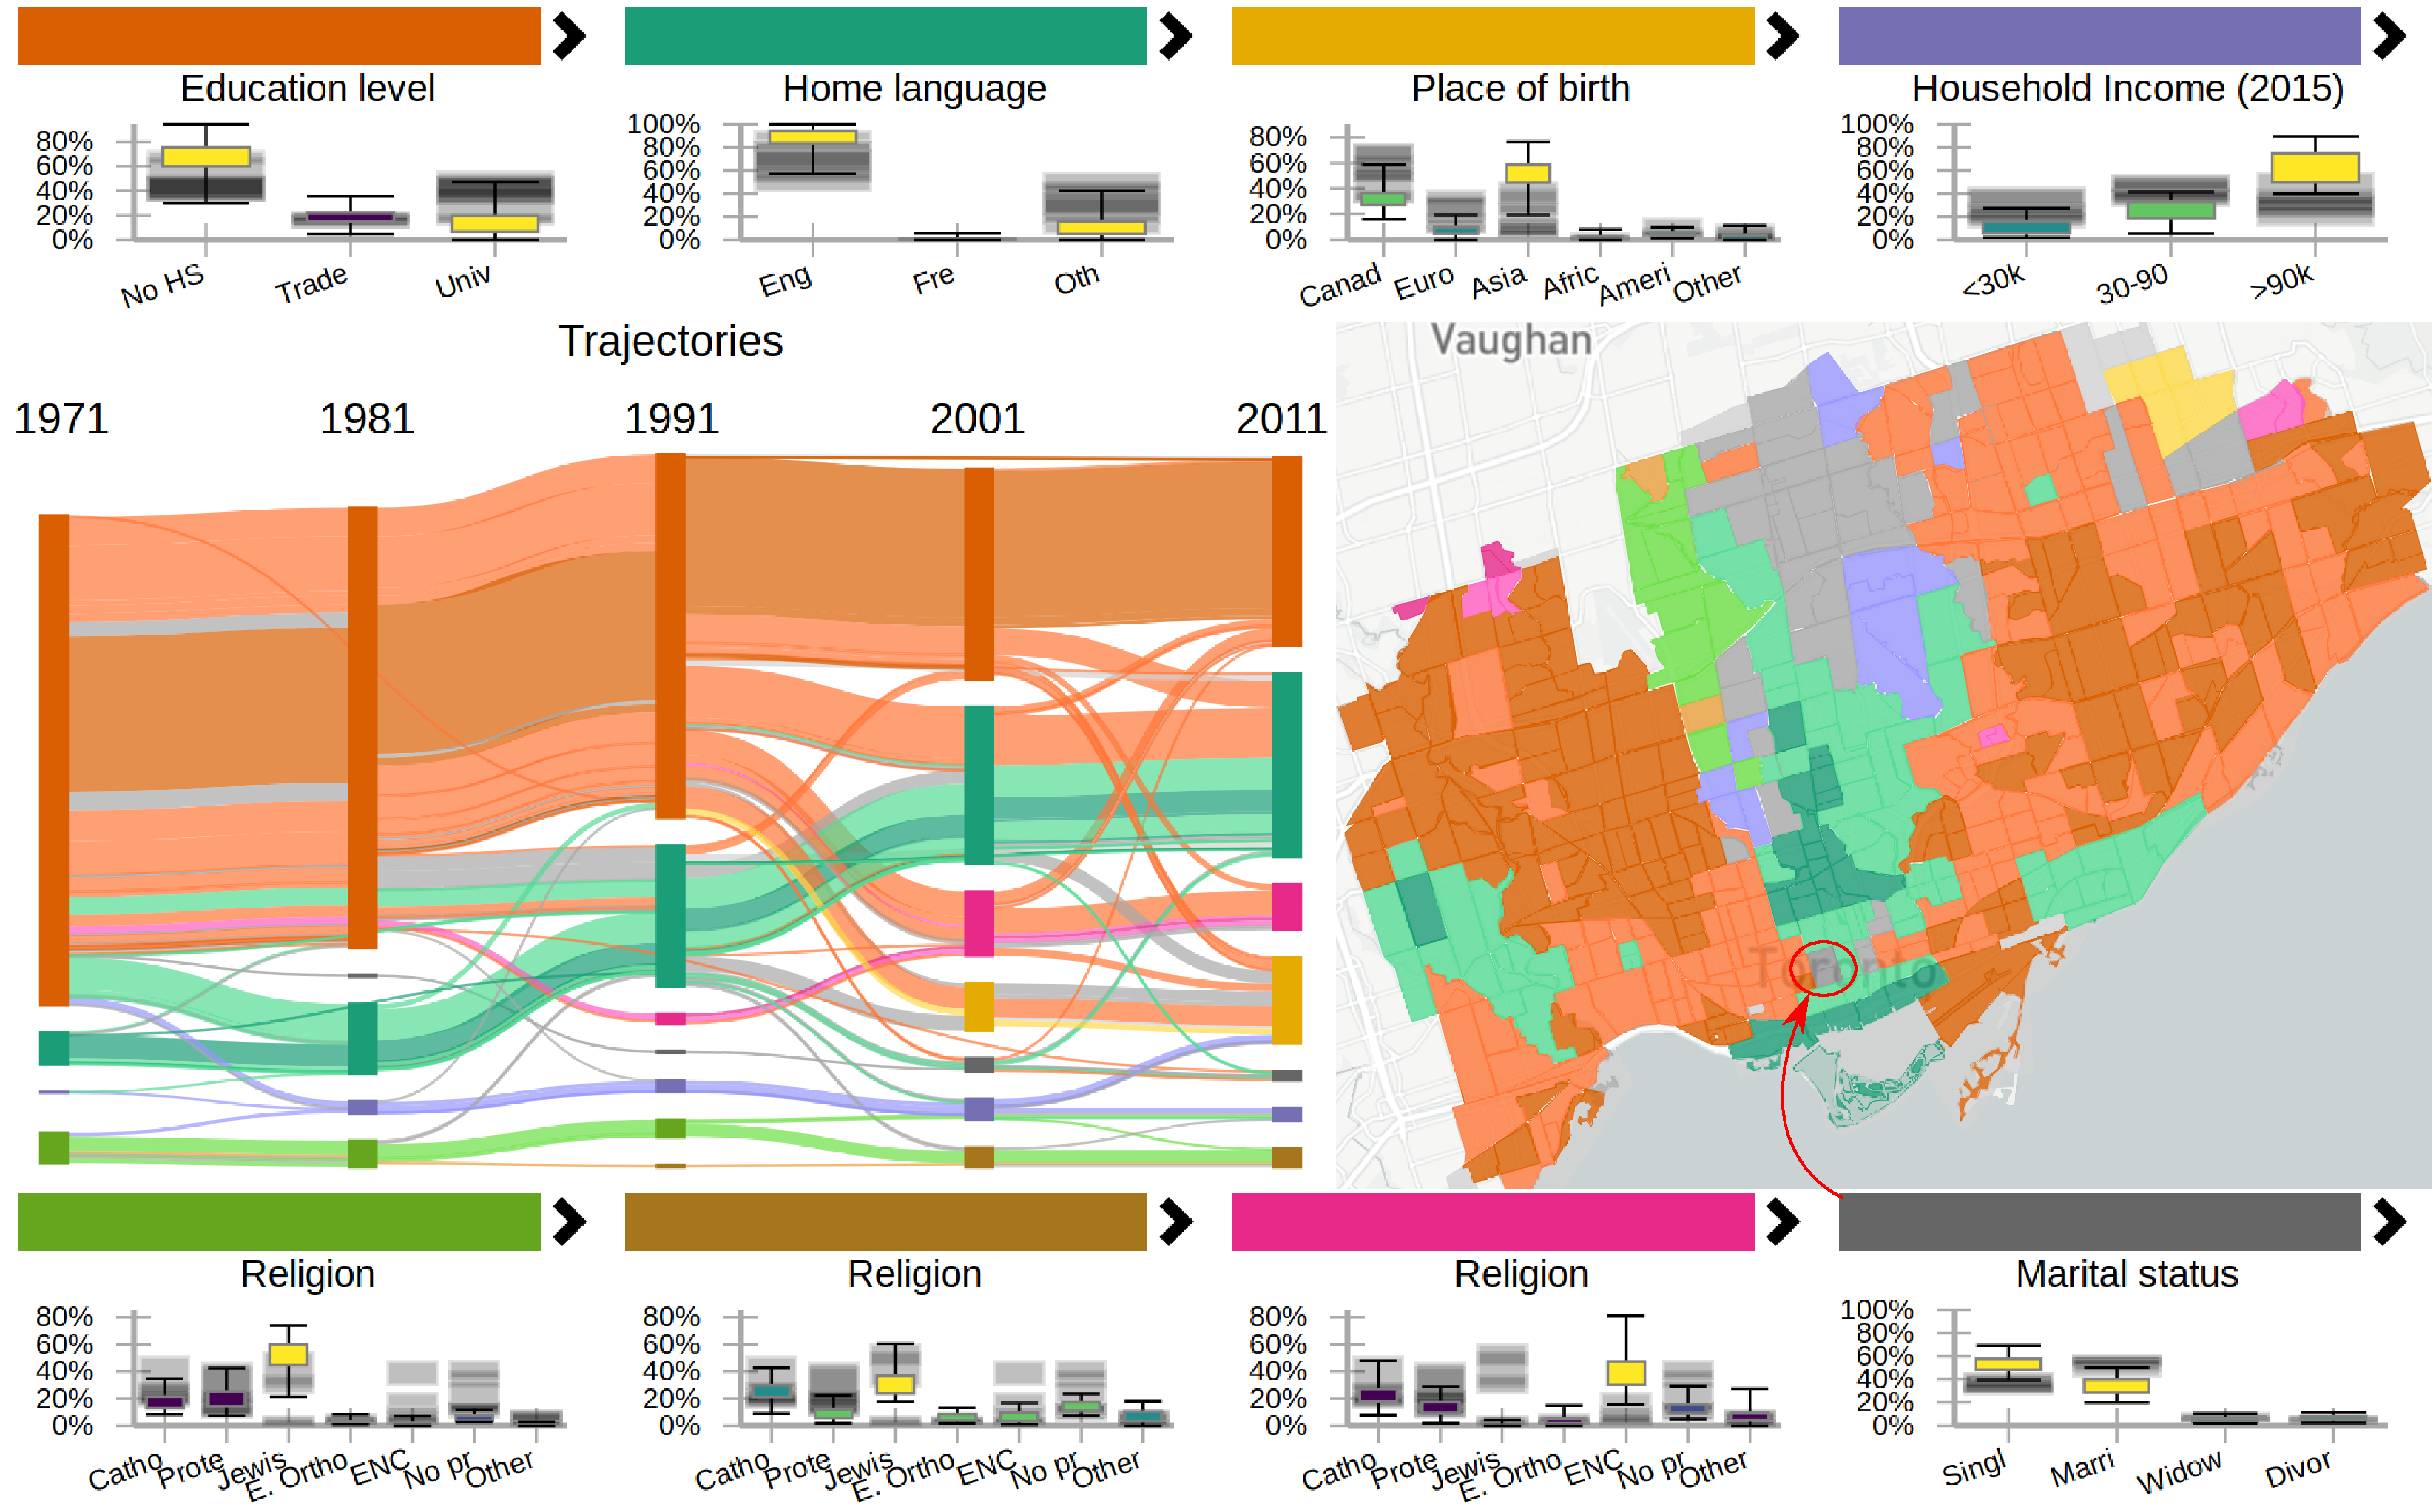
\includegraphics[width=0.85\linewidth]{to.pdf}
    \caption{Clustering results for Toronto, with eight clusters, including
    clusters representing Jewish population, high and low income, low education,
    and Asian immigration.\label{fig:to}}
\end{figure}

We again are guided by the four questions embedded in the interface: what, how,
where, and who. The boxplots address what clusters defined Toronto over this
period. The population with low percentage of University degrees is represented
in orange, mostly anglophone population in green, Asian immigrants in yellow,
high percentage of income in the highest bracket in purple, high percentage of
Jewish people in light green and brown, high percentage of Eastern Non-Christian
religion in pink, and high concentration of single people in dark grey. 

From the trajectories plot, we can see how the city changed. It shows that
Toronto is more dynamic than Chicago, with one cluster constantly shrinking. In
the 1970s, the city was divided into four clusters: low number of university
degrees, Jewish population, majority anglophones, and high income.
Interestingly, the more recent clusters that absorbed regions from the orange
cluster have similar education profiles and are differentiated by other aspects.
In this sense, the city is growing diverse, changing from a common low education
profile to a higher level of education with more diversity in religion (pink)
and immigration (yellow). Indeed, the growing Asian population is visible
starting in the 1980s and building thereafter, leading to the yellow and pink
clusters. While both include a high percentage of people born in Asia, the pink
is more defined by religion, with low percentage of university degrees, and
contains the lowest percentage of people in the highest income bracket for these
clusters; the yellow is less defined by religion, and has higher education and
income, geographically corresponding to the Markham region, know for its Chinese
population. A similar division also happens for the two Jewish clusters, where
the light green cluster has lower education and income levels than the brown
cluster. The purple cluster of high income is somewhat stable. Until 2011 the
cluster included the Bridle Path neighbourhood, known for its wealthy
population. In 2011 it was classified into the yellow cluster of Asian
immigration, since about 40\% of the population for this CT were then born in
Asia. The income distribution did not change, with 85\% of the population with
an income of 90k CAD or more.


Examining where and by whom these changes occurred reveals additional
information about the city's underlying dynamics. The most significant indicator
of Toronto's dynamism is the presence of grey regions on the map. These
represent regions associated to three or more clusters over this five census
period. Using the 'Add' mode for the trajectory selection, we select their
trajectories, and a subset of the details is illustrated in
Figure~\ref{fig:toVol}. These regions account for about 5\% of Toronto's
population. The whole region was classified into the orange cluster in 1971 (low
level of university degrees). By 1991, most of the region was classified into
the green cluster, representing anglophone population, mostly Canadian born,
with a higher level of education. As the corresponding plot indicates, this
trend in increasing education is city-wide, but this region has people with
better education than most. In 2001, the purple cluster of high income annexes
neighbouring parts of the volatile region, and the Asian born population
increases sharply, as illustrated by the appearance of the yellow cluster.  This
cluster indicates well educated, higher income, and about 30\%-50\% Asian born
population. By 2011, the yellow cluster increased considerably, annexing parts
of the high income purple cluster, including the neighbouring Bridle Path area.

\begin{figure}
    \centering 
    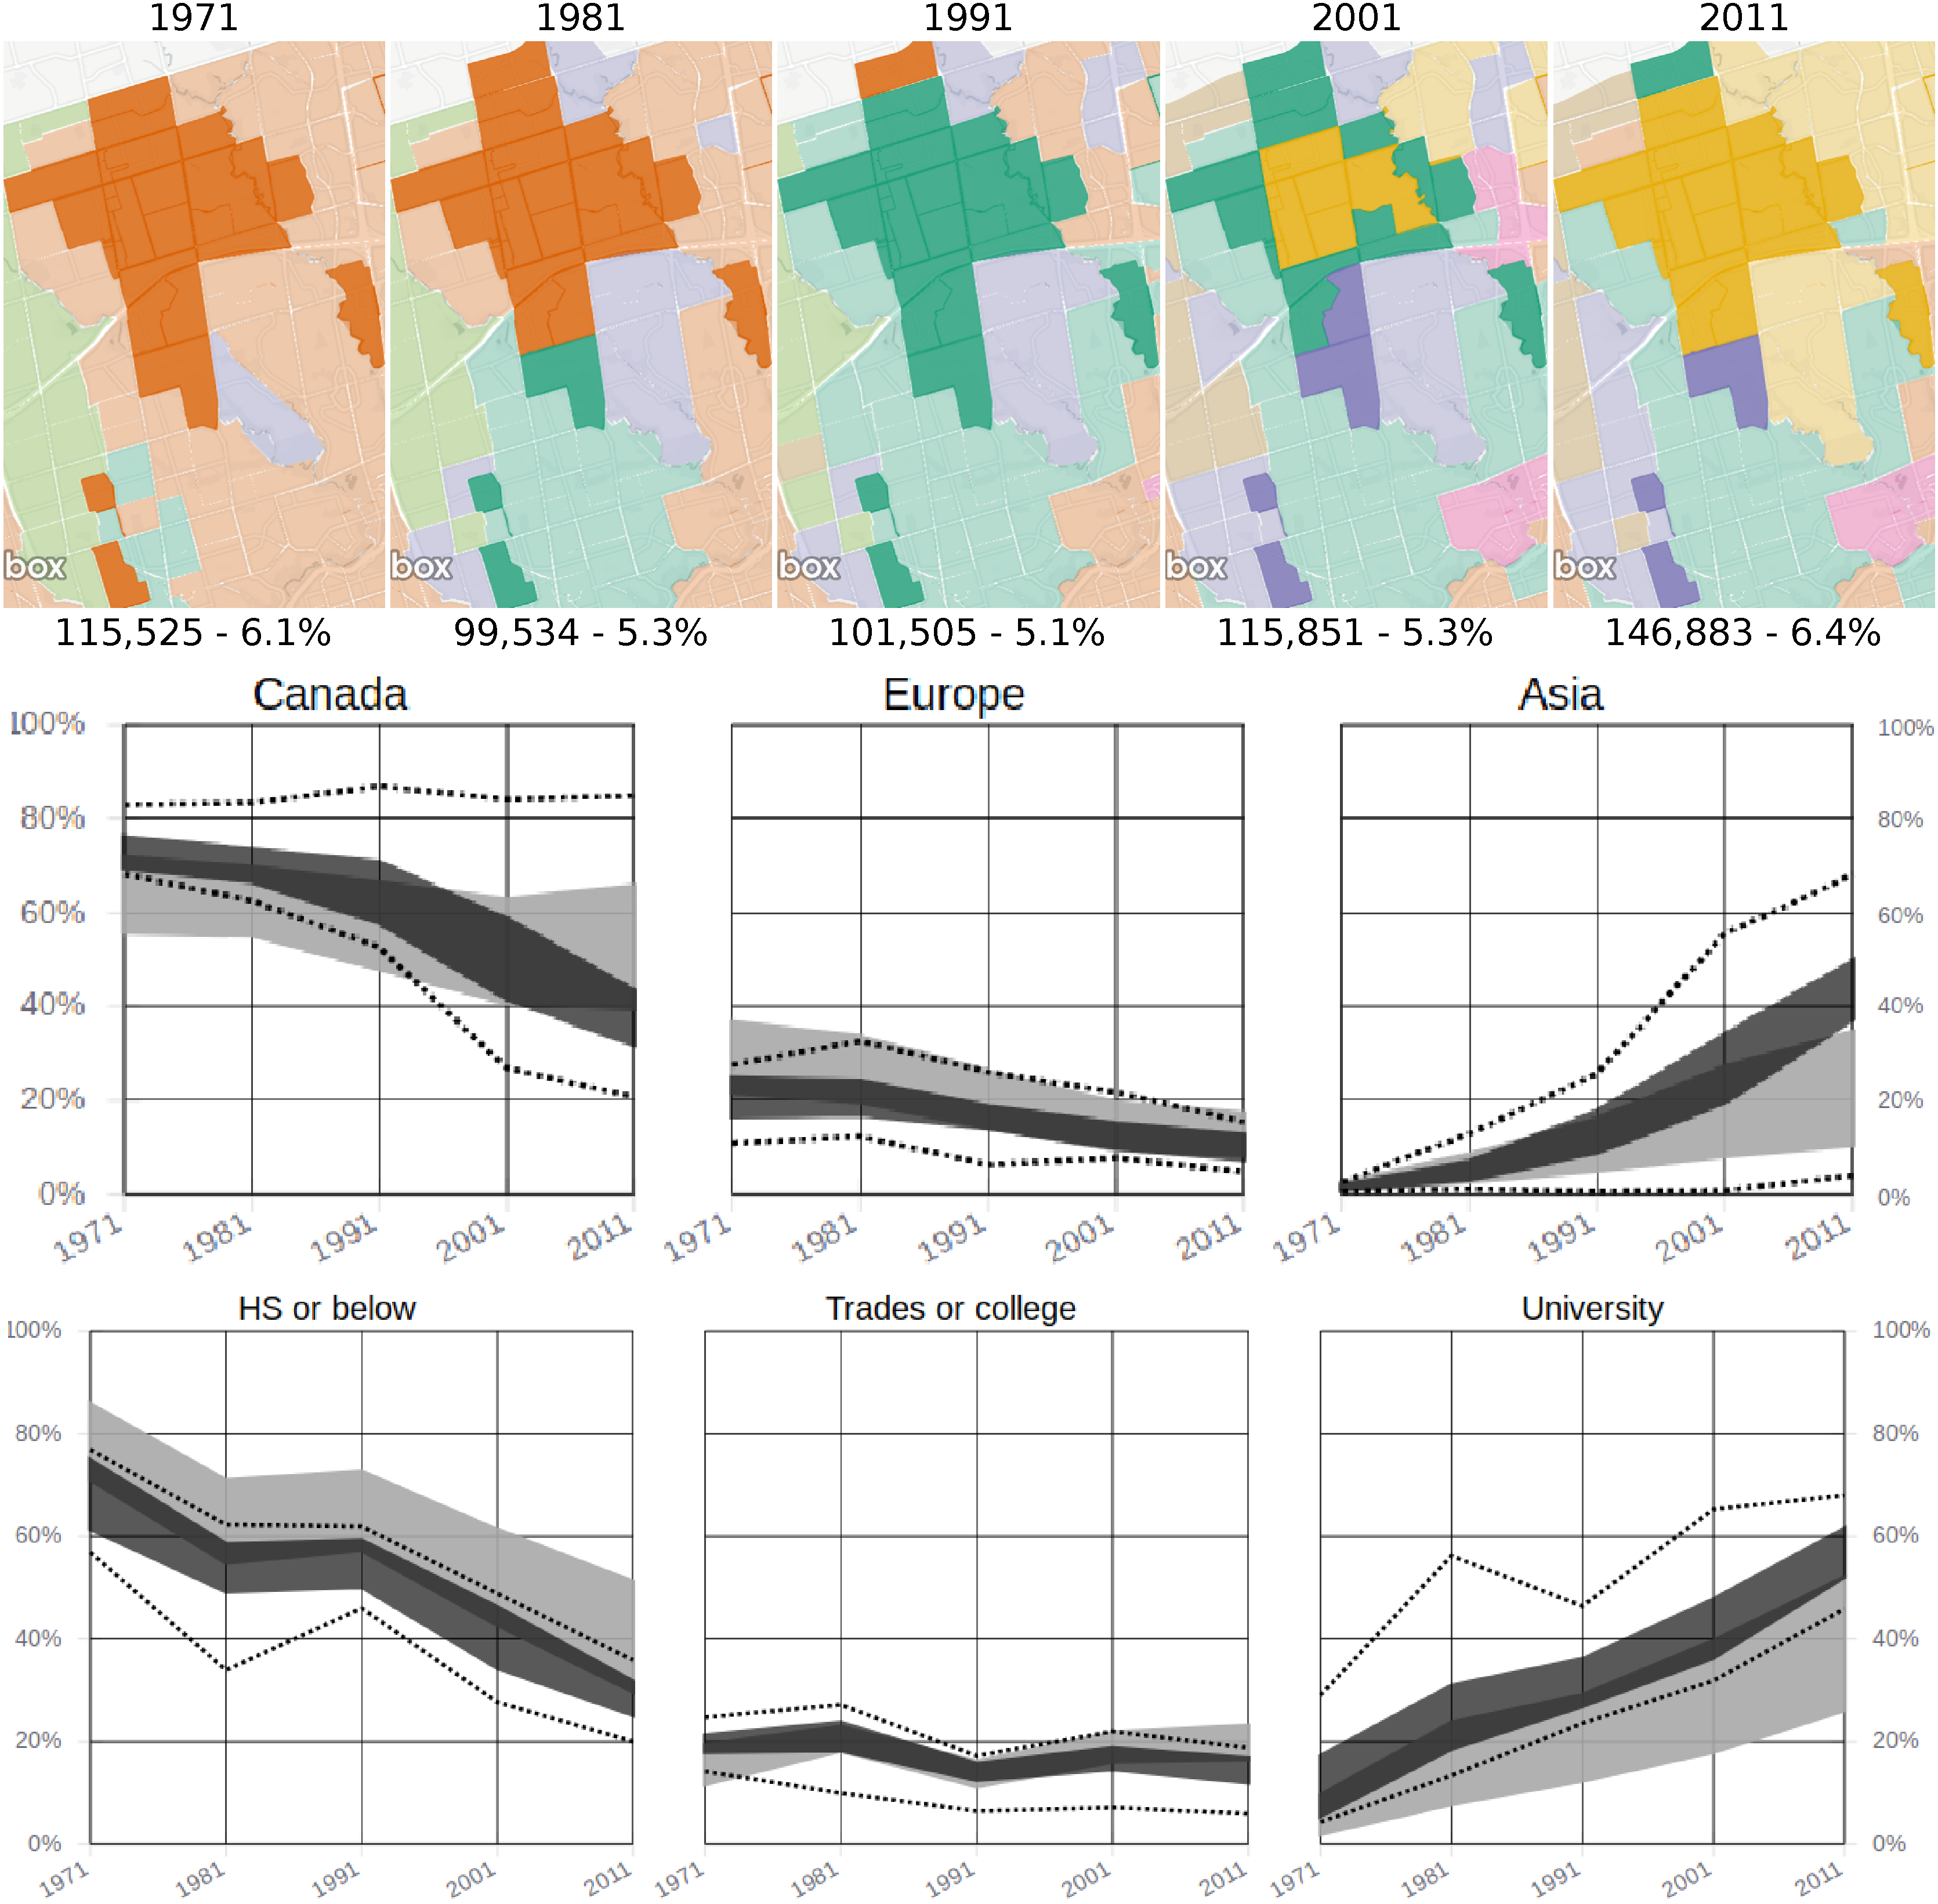
\includegraphics[width=0.75\linewidth]{toVol.pdf}
    \caption{Details for some regions of Toronto that were classified into 3 or
         more clusters over time.\label{fig:toVol}}
\end{figure}



The geographical borders of the clusters obtained using our method are similar
to the regions presented by previous studies considering
Toronto~\citep{hulchanski2007three}. However, our interface provides a deeper
insight into their demographic composition, since we consider more data than
solely Average Income, which appears to be a good proxy variable nonetheless.
This scenario showcases the ability of our method and interface to capture and
understand the sources of urban volatility.

\section{Expert feedback}
\label{sec:expert}
As our method and tool are novel to the field, and somewhat exotic,  we
subjected them to the critical scrutiny of experts. We contacted academic and
industry experts in sociology and urban sciences to solicit their evaluation of
our methodology. They had access to the prototype tool, a descriptive
documentation of the features (included in the supplementary material), and a
sequence of documentation videos illustrating how to perform specific tasks. The
documentation explains which datasets are used and how the data is represented
and processed, noting explicitly that there is no geographic harmonisation. We
focused our inquires on the results obtained, asking if they found anything
interesting in the data. The message sent and their full response is included in
the supplementary material. Each of the five experts is identified by a letter,
from A to E. 



The overall overall response of the experts was positive,  mentioning that the
prototype allows them to analyse census data without the additional work of
obtaining and cleaning the data (A, B, E), and it allows the inclusion of
geographic visual analysis tools in their research process (D). It enables the
users to tell different stories about neighbourhoods/cities and their changes
(A), visualise the relationship between key urban variables over time (D),
offering a quick way to identify particular neighbourhoods that one may be
interested in studying more in depth around a particular issue or efficiently
understanding the context of an area (E).  Indeed, the experts identified
gentrification processes in Manhattan (B) and Dallas (E), reinforced a
hypothesis for occupational clustering (D), and highlighted how the method can
be used to compare neighbourhoods and cities (A). In summary, their view was that
the proposed methodology can be a viable alternative for the visual analytics of
evolving demographic data.



The interface was "easy to navigate" (B), but it was also considered
"overwhelming" (A), "intimidating" (E), and "tricky to interpret" (C), possible
side-effects of our effort to increase  representational accuracy, where we
avoided using simplified representation or labels. Identifying clusters by their
most relevant variables was welcome, but the overlap of information from
different clusters in the boxplot was "a bit confusing" (C) when colour was not
present. Further, most clusters can be sufficiently characterised using only the
most relevant aspect, but this is not generally true. 


While the map of trajectories was mentioned as a "good summary map", how it
related to the clustering method was unclear (C). The methods include different
options on how the colours are used, but both are works in progress since reliably
representing several distinct entities using colours is humanly unfeasible.
Indeed, the number of distinguishable colours was a significant constraint, we
found indications that more clusters should be used in some cases, even if eight
clusters is more than what is traditionally considered in these analyses.
Conversely, increasing the number of clusters would also complicate the
interpretation of the results.


The experts also mentioned the poor responsiveness of the method when changes in
the clustering parameters required server-side processing (B,D). Indeed, the
current implementation can take a few minutes to cluster regions with high
number of CTs, like Los Angeles or Brooklyn. Server-side processing reduced the
amount of data transferred to client, but it might increase the response time
under load. We implemented a caching policy, but fully pre-processing the
results is not practical due to size of the parameter space.

Most of the experts demonstrated interest in using our method in their research
(A, B, D, E), aiming to use the census data as a backdrop for other datasets,
providing demographic context. They also mentioned the need to export subsets of
data, plots, and maps to be used in reports and publications (C, D, E). More
importantly, while these experts were aware that our method does not perform
geographic harmonisation, none of them mention it. We did not specifically ask
if this difference led to unexpected results, but rather if they found
interesting insights. 